\section{Data preparation}

Once the dataset is captured and stored, the data still has to be formatted and prepared to be fed to our models. We decided to alter the recordings as little as possible, since it is very valuable to have raw data in projects like this one. This means any modification of the data is done at runtime. This section describes the formatting and preprocessing applied to the datasets.

\subsection{Environment}

We used python to work with our datasets and to write the models described in next section. Visualizations were done in \texttt{Jupyter notebooks} using \texttt{matplotlib}. Data processing was achieved in a python project using \texttt{numpy} to read and manipulate the data and \texttt{scipy}'s signal processing library.

% -------------------------------------------------------------------------------------------------------------
\subsection{Data partitioning}

\subsubsection{Raw partitioning}

Our first approach with the datasets was to segment each recording in windows of size $n$. In order to be able to tune the window size and to see its impact on the performance of the model, we made it a parameter.

The result for each tag is an array of windows, each comprised of $n$ complex samples. If the number of samples in a tag's recordings is of size $L$, then this array contains $L/n$ windows. An example of a resulting window can be seen in figure \ref{fig:window}.

\begin{figure}[htbp!]
  \centering
  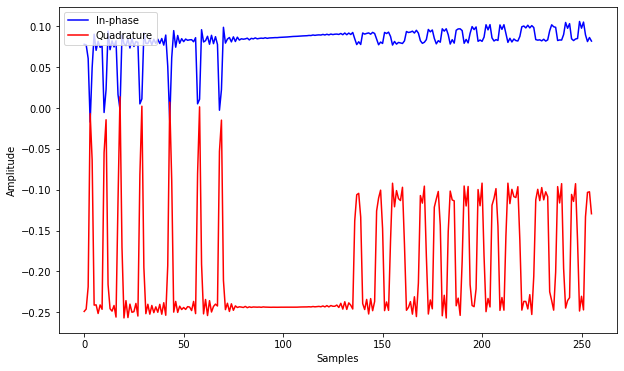
\includegraphics[scale=0.55]{figures/dataprep_window.png}
  \caption{Visual example of a window of size $n = 256$}
  \label{fig:window}
\end{figure}

\subsubsection{Detecting communications}

It was soon clear that feeding the raw data without at least selecting segments that actually contained communications would not yield fantastic results. Indeed, most windows would contain only the carrier signal generated by the reader. These long segments of the signal contain little to no meaningful information. This is why we used peak detection algorithms to detect actual communications and filter out the uninteresting parts of the signal.

When experimenting with the first dataset, we used the \texttt{signal.find\_peaks} function from the \texttt{scipy} library. It allowed us to specify a minimum required height for a peak to be considered as well as the minimum required \textit{prominence} of the peak. (The prominence defines the height of a peak relative to the lowest contour lines around it that don't include higher peaks \cite{wiki_prominence_2020}.) This allowed us to detect, peaks from all of the transactions in the signal, with almost no false positives. We could then create our windows as decribed in the section above, using some peaks as the start of our windows, in a similar fashion as \textcite{youssef_machine_2017} did in their work.

\begin{figure}[htbp!]
  \centering
  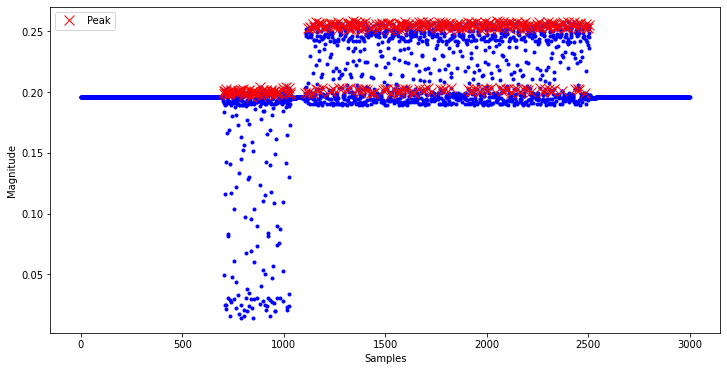
\includegraphics[scale=0.55]{figures/dataprep_peaks.png}
  \caption{Visual representation of the peak detection on an NFC transaction}
  \label{fig:peaks}
\end{figure}

When our second dataset came into play, it became clear that calculating the prominence was computationally too expensive for data of this size. Using the more common \textit{threshold} parameter, which is the vertical distance of a point to its neighbours, worked just as well for our needs and performed about 220 times faster (1min 21s vs 365ms, on our system). It should have been obvious from the description of these characteristics that prominence was a lot harder to calculate, but it didn't occur to us initially.

Using windows of length 256, the total number of windows in dataset 2 is 32'168 (4021 for each tag, as the number of window is balanced between classes). We considered augmenting our dataset using sliding windows which overlap, as \textcite{riyaz_deep_2018} propose, but couldn't find the time in the scope of this project. This would considerably expand the dataset's size and potentially bring superior shift invariance to the model. This is an interesting idea to explore further.

\newpage
\subsection{Input formatting}

Once our data is filtered and partitioned for input, the question of the format comes up. Indeed, a machine learning model will not accept complex numbers as input without adapting the loss function. This can be done without great difficulty, but most of the research we considered preferred representing the data as a two-dimensional array comprised of two float arrays: one for the real parts and the other for the imaginary parts. Figure \ref{fig:2din} shows a representation of the input after the windows were created and formatted this way.

\begin{figure}[htbp!]
  \centering
  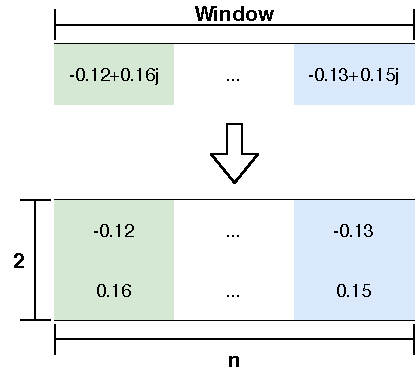
\includegraphics[scale=0.8]{figures/dataprep_2d.pdf}
  \caption{Format for the two-dimensional input}
  \label{fig:2din}
\end{figure}

For our experiments with SVMs, such a representation wasn't appropriate since SVMs don't accept multidimensional inputs. This is why we propose two formatting options: "2D" for the neural networks and "1D" for the SVM. The latter appends the array containing the imaginary parts to the array containing the real parts, as shown in figure \ref{fig:1din}.

\begin{figure}[htbp!]
  \centering
  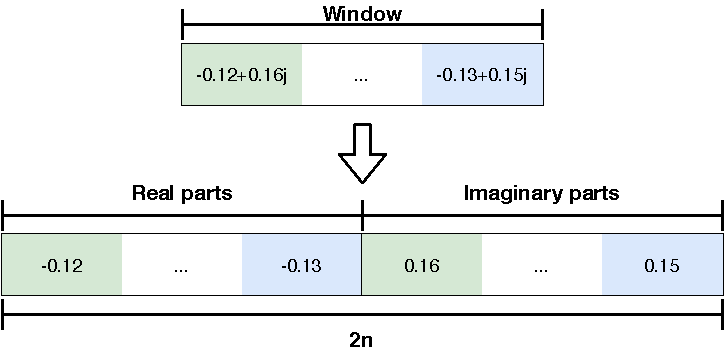
\includegraphics[scale=0.8]{figures/dataprep_1d.pdf}
  \caption{Format for the simple input}
  \label{fig:1din}
\end{figure}

% -------------------------------------------------------------------------------------------------------------
\subsection{Normalization}

Normalization is the action of changing the scale of numerical values in a dataset to a common range. It is essential in some machine learning applications, as it ensures one type of features won't have a greater effect on the different parameters of a model than another.

Of course, we don't have many different features with different scales in our dataset, so normalization is not absolutely essential here. However, there are amplitude differences between our recordings and making sure every sample stays in a set range will help the neural network converge faster. Here, we chose the range $[-1, 1]$ for our values, as they already oscillate around 0 by nature.

% -------------------------------------------------------------------------------------------------------------
\subsection{Splitting into training, testing and validation datasets}

Another very common operation in data preparation for machine learning purposes is randomly splitting the data into three separate sets.

\begin{itemize}
  \item The \textit{training set} is usually the biggest chunk of the dataset. It is fed to the model in batches for it to train itself to associate an input to an output.
  \item The \textit{validation set} is the data we can use to monitor the performance of the model at each training iteration. We give this data to the training algorithm, but it doesn't use it to train the model. Instead, it uses it to validate the model's performance after each epoch. We can use the information given by the validation predictions to tweak the model's parameters. This is also the data we monitor to perform "early stopping".
  \item The \textit{testing set} is used once the model is completely trained. As it has never been used before, neither by the model, nor by you before you tweaked the parameters, it can be used as an unbiased benchmark of the finished model.
\end{itemize}

In this project, we chose to separate our dataset as follows: 70\% for the training set, 20\% for the validation set, and 10\% for the testing set.
